\documentclass[11pt]{article}
\usepackage[margin=1in]{geometry}
\usepackage[T1]{fontenc}
\usepackage{lmodern}
\usepackage{microtype}
\usepackage{hyperref}
\hypersetup{hidelinks,hypertexnames=false}
\usepackage{booktabs}
\usepackage{tabularx}
\usepackage{amsmath,amssymb}
\usepackage{enumitem}
\usepackage{graphicx}
\usepackage{float}
\usepackage{algorithm}
\usepackage{algpseudocode}
\graphicspath{{../shared/figures/}}
\title{Resource-Versioned Outcome-Aware Metacontrol for Software Action Systems}
\author{Felipe Santib\'a\~nez-Leal\\CAOS open-research programme}
\date{}
\newcommand{\doctype}{Preprint}
\newcommand{\docversion}{v0.02}
\newcommand{\docdate}{30 October 2026}
\newcommand{\versiondoi}{10.5281/zenodo.23821087}
\newcommand{\conceptdoi}{10.5281/zenodo.23784117}
\newcommand{\docrepo}{github.com/fsantibanezleal/CAOS\_Neuraxis}
\newcommand{\headerblock}{%
\begin{center}\fbox{\parbox{0.94\textwidth}{\small\raggedright
\textbf{\doctype} \quad$\cdot$\quad \docversion, \docdate \quad$\cdot$\quad Licence CC BY 4.0\\[2pt]
CAOS open-research programme \quad$\cdot$\quad Neuraxis, software-action metacontrol\\[2pt]
Version DOI \href{https://doi.org/\versiondoi}{\texttt{\versiondoi}} \quad$\cdot$\quad concept DOI (always latest) \href{https://doi.org/\conceptdoi}{\texttt{\conceptdoi}}\\[2pt]
Not peer reviewed. Source code, data and computational records: \href{https://\docrepo}{\texttt{\docrepo}}
}}\end{center}\vspace{4pt}}
\begin{document}
\maketitle
\headerblock
\begin{abstract}
Software agents must choose admissible actions quickly while deciding whether uncertainty, novelty, or anticipated consequences justify slower computation. We specify a resource-versioned, outcome-aware metacontroller (M12) that combines recurrent action preference, bounded model-based lookahead, outcome-sensitive delegation, explicit surprise detection, asynchronous planner proposals, and validation against current resource revisions. We give its decision contract, state transitions, allocation objective, and falsifiable evaluation protocol, then report the existing matched benchmark evidence. On 1,200 core episodes, M12 solved 1,160 while a guarded finite-state controller solved 1,200; median decision latencies were 18.13 ms and 0.0219 ms, respectively. Four component ablations matched M12 task success, and the fitted deferral gate selected never-defer. On 24 structural-transfer episodes, XGBoost solved 24 and M12 solved 21. A separate 1,536-episode semantic-transfer lane records 38/128 successes for M09, 18/128 for M12, and 2/128 for M04; M12 loses 22 paired cases and wins two against M09. Thus this implementation has not shown a task-success or efficiency advantage. The paper contributes a concrete method specification and a negative result that identifies where the allocation hypothesis remains untested.
\end{abstract}
\noindent\textbf{Keywords:} metacontrol, learning to defer, software agents, resource versioning, asynchronous planning, negative results

\section{Introduction and problem formulation}
Let a software environment at decision time $t$ expose observation $o_t$, candidate set $A_t$, and a vector of resource revisions $v_t$. A fast controller selects an admissible action $a_t\in A_t$ from a typed action contract. A deliberative planner may return a proposal after the environment changes. The controller must both select actions and decide when additional computation is worth its cost. We distinguish (i) authority, enforced by the action broker, from (ii) policy quality, measured by environment outcomes. A valid proposal is not necessarily useful; a useful proposal is not admissible unless it satisfies the current contract.

The distinction matters because software tasks combine two different sources of uncertainty. The controller may be unsure which action is likely to satisfy a goal, while the executor may independently know that a candidate is forbidden, malformed or stale. More computation can reduce the first uncertainty, but it cannot relax the second constraint. A planner may produce a coherent answer for a previous file version, a prior process state or an expired user goal. Applying that answer because it sounds plausible converts uncertainty about the world into an unreviewed side effect. The controller must therefore arbitrate computation under a separate, current-state action authority boundary.

We study the decision problem as an episode with a declared goal predicate, a sequence of observations, a changing set of registered candidates, and a deadline and resource budget. The episode terminates when the independent checker accepts the postcondition, a terminal failure occurs, or a declared resource bound is reached. Neither a valid JSON response nor a broker effect record implies task completion. This distinction makes the question falsifiable: the proposed method must improve measured task or cost outcomes under a fixed action/effect contract; architectural complexity, confidence scores and planner text are not outcome evidence.

The central question is whether outcome-aware, stateful allocation can improve the joint frontier of task completion, decision latency, deliberation cost, and effect correctness relative to fixed fast policies and fixed delegation. The hypothesis is conditional: for environments with consequential uncertainty and variable tool behavior, a controller that predicts incremental value and invalidates stale proposals may outperform fixed policies under a matched budget. The current benchmark does not instantiate enough consequential uncertainty to establish that claim.

This study has three contributions. First, it defines a concrete action-selection and deliberation interface in which candidate ranking, effect admission, asynchronous proposal validity, and final goal verification have separate owners and records. Second, it specifies an outcome-aware controller with recurrent preference, bounded learned-model lookahead, an incremental-utility gate, and resource-revision binding, including the assumptions under which each check has meaning. Third, it reports the frozen benchmark evidence without converting implementation detail into a performance claim: the proposed controller loses to the guarded rule baseline on core success and latency, fails a concentrated cancellation subset, and does not change success under the tested ablations. The report is organized from prior work and formal problem statement through method, theory, protocol, results, ablation, discussion, limits, and reproducibility. All numerical claims refer to the hash-checked artifacts named in the companion report; structural and semantic transfer are different populations and are never added to the core denominator.

\section{Related work}
Dual-controller accounts distinguish cached or habitual responses from model-based planning, while computational accounts study arbitration as a function of uncertainty and the relative reliability of model-free and model-based values \cite{daw2005,lee2014,kool2016}. These findings motivate functional analogies, not a claim that a software controller reproduces neural mechanisms. Predictive-processing and recurrent-control theories offer candidate descriptions for residual-driven adaptation and persistent state \cite{rao1999,mante2013}. Biological evidence does not determine the software architecture or validate its performance.

Machine-learning systems that defer to experts frame delegation as a selective prediction problem with a cost-sensitive decision boundary \cite{madras2018,mozannar2020}. Rational metareasoning treats computation itself as an action whose expected value must be weighed against its cost \cite{russell1991}. Hierarchical reinforcement learning supplies temporal abstractions for policies whose actions persist over multiple environment steps \cite{sutton1999}. These approaches typically evaluate the deferral decision or learned computation policy; the proposed controller adds explicit resource-revision validity and observed planner outcomes to the action-level loop. Asynchronous agent architectures and tool-use benchmarks provide complementary engineering and evaluation precedents, but are not direct replications of the present benchmark \cite{dptagent,toolsandbox}.

Language-model tool-use methods such as ReAct and Toolformer interleave or learn calls to external APIs, while SWE-bench evaluates issue resolution in real codebases and tau-bench places tools in changing, multi-turn user settings \cite{react,toolformer,swebench,taubench}. These works establish that interaction requires more than answer fluency, but their objectives and environments differ from candidate selection under resource revision. They are precedents for stateful evaluation, not numerical comparators. Direct comparisons would require identical tasks, candidate exposure, tools, effect authority, model availability and evaluation oracles.

The present system also separates an asynchronous planner proposal from the broker's effect decision. A planner call may run concurrently with a fast controller; this can hide part of its latency, but background compute and completions still consume resources. Reporting only apparent fast-path latency would conceal the work spent and the possibility that the answer arrived after its assumptions expired. We therefore retain request, completion, proposal-use, invalidation and effect events as separate outcomes. This accounting is compatible with direct synchronous planning but does not make the policies equivalent: their information timing and number of decisions differ.

Several prior metareasoning formulations optimize which computation to execute next, while learning-to-defer formulations estimate when an external expert should replace a base predictor. The current controller is not a complete solution to either theoretical problem. Its gate is a fitted finite-data approximation to paired incremental utility; it has no guarantee under arbitrary distribution shift. Its revision check is an operational validity invariant, not a proof of end-to-end safety. These limits set the claim boundary and motivate treating the results as an empirical test of one implementation rather than confirmation of a general theory.

The comparison methods are drawn from distinct learning regimes and should not be collapsed into one category. Logistic imitation estimates conditional action preference from labeled states; gradient-boosted trees model nonlinear feature interactions; a gated recurrent unit adds bounded hidden state; a contextual bandit learns from action-conditioned feedback; proximal policy optimization updates a stochastic policy from reward-bearing trajectories; and learned-model lookahead uses a transition approximation to score candidate sequences. Their feedback, observability, and sample requirements differ. Neuraxis exposes these methods under a common candidate and broker contract while retaining distinct training signals and histories. This paper focuses on the proposed controller and compares measured outcomes only within each declared population \cite{friedman2001,chen2016,cho2014,li2010,schulman2017,suttonbarto2018}.


\section{Theory and method properties}
Let $G$ be a goal predicate over final environment state and $J(\pi)$ the expected task utility when controller $\pi$ acts through a fixed runtime and action contract. A computation policy chooses both a physical action and, when permitted, a metalevel action such as requesting a planner result or refreshing an observation. An exact solution would require a model of environment transitions, computation outcomes, latency and interactions among candidate actions. The implementation uses learned predictors and a threshold gate instead; its decision rule is approximate and inherits the coverage and misspecification limits of its training data.

A planner call has positive decision value only when its expected improvement in final task utility exceeds its full cost. For a computation $q$ with returned information $Z_q$, define
\begin{equation}
\operatorname{VOC}(q\mid o_t)=\mathbb{E}\!\left[\max_a U(a\mid o_t,Z_q)\right]-\max_a U(a\mid o_t)-C_q .
\end{equation}
Here $C_q$ includes compute, latency, queue occupancy and opportunity cost. This value is nonnegative only when the information can be used before the deadline and is evaluated under the same goal and resource state. If the answer arrives after a consequential resource change, its value may be negative even when it was accurate at request time.

The fitted gate estimates a score $g_\psi(x)$ from paired outcomes and delegates when that score crosses a selected threshold $\tau$. The gate and threshold are distinct fitted objects. Their finite-sample errors affect false delegation and missed delegation. A threshold above observed score support creates a deterministic never-defer policy; it does not show that planner use has zero population value. A calibrated risk claim would require a held-out risk/coverage analysis, enough positive and negative examples and a prespecified target. The current data do not establish such a guarantee. Probability calibration is separate from ranking quality \cite{guo2017}.

The version-binding design supplies a narrower conditional property. Suppose a request is made from canonical binding $B_t$ with digest $\beta_t=H(B_t)$. If canonicalization is deterministic, the digest is collision-resistant for the declared threat model, and the executor independently recomputes resource revisions, then a proposal with a different binding is rejected before execution. This argument assumes that the binding is complete, revision sources are reliable and the final admission path cannot be bypassed. It does not show that a proposal is optimal, that an effect is reversible, or that external changes are all observable.

\begin{equation}
\Pr(\text{stale proposal admitted}\mid\text{all bound revisions observable and broker check active})=0
\end{equation}
is a runtime target under explicit assumptions, not an estimate from the task-success benchmark. An empirical report of zero invalid admissions must state the number and kinds of attempted stale proposals; if a test contains no stale proposals, it supplies no bound on admission risk under changing state.

The objective is retained as a vector rather than collapsed into an undocumented scalar:
\begin{equation}
\mathbf{Y}=(Y_{\mathrm{goal}},T_{\mathrm{decision}},T_{\mathrm{episode}},C_{\mathrm{compute}},N_{\mathrm{calls}},E_{\mathrm{incorrect}}).
\end{equation}
The entries denote verified completion, policy-decision and full-episode time, compute cost, planner-call count and incorrect effects. A composite utility can be useful in a concrete deployment, but its weights must be fixed before evaluation and justified by the task owner. Reporting component outcomes allows readers to distinguish a fast but unreliable controller from a slower complete one.

For a scalar endpoint such as success, uncertainty must respect assignment and dependence. Let $Y_{fvs}$ be the outcome for task family $f$, variant $v$, and seed $s$. A family-cluster procedure would resample families and retain all nested observations from each selected family. The archived suite is not a probability sample of families, so even that interval would remain conditional on its authored set. The seed-cluster bootstrap used for the frozen report is degenerate for repeated deterministic cells. A percentile interval is
\begin{equation}
[L_{.025},U_{.975}]=[Q_{.025}(\widehat{\theta}^{*}),Q_{.975}(\widehat{\theta}^{*})],
\end{equation}
where $\widehat{\theta}^{*}$ is recomputed for each resampled cluster sample. If every resample yields the same statistic, the collapsed interval describes archived variation, not certainty about an unobserved target population. This distinction is central to interpreting the negative result \cite{efron1993,demsar2006,nadeau2003}.

For any scalar endpoint such as success, uncertainty must respect the assignment and dependence structure. If $Y_{fvs}$ is an outcome for family $f$, variant $v$, and seed $s$, a family-cluster procedure would resample families and retain all nested observations from each selected family. The archived suite is not a probability sample of families, so such an interval would remain conditional on this authored set. The seed-cluster bootstrap used for the frozen report is degenerate for repeated deterministic cells. In general, a percentile interval is
\begin{equation}
[L_{.025},U_{.975}]=[Q_{.025}(\widehat{\theta}^{*}),Q_{.975}(\widehat{\theta}^{*})],
\end{equation}
where $\widehat{\theta}^{*}$ is recomputed for each resampled cluster sample. If every resample yields the same statistic, $L_{.025}=U_{.975}$ describes the archive's variation, not certainty about an unobserved target population. This distinction is central to the negative interpretation here \cite{efron1993,demsar2006,nadeau2003}.

The proposed controller has no unconditional performance guarantee. Such a guarantee would require assumptions about model calibration, counterfactual branch comparability, environment drift, planner quality, revision observability and broker correctness. The frozen benchmark has a deterministic guarded controller that solves every core task, and many repeated seeds preserve identical outcomes. This section states conditional interface properties; it does not prove a regret bound or safety theorem for arbitrary software environments.

\section{Method: resource-versioned outcome-aware metacontrol}\label{sec:m12}
\subsection{Controller state and fast action score}
The controller maintains bounded episode-local recurrent state $h_t$, a residual statistic $r_t$, the latest resource revision vector $v_t$, and at most one active planner request. A recurrent policy emits candidate probabilities $p_\theta(a\mid o_t,h_t)$. A learned transition model supports bounded lookahead utility $U_\phi(a\mid o_t)$ over the same admissible candidates. The implementation combines these signals as a ranking score, not as a calibrated probability:
\begin{equation}
S_t(a)=\log(p_\theta(a\mid o_t,h_t)+\epsilon)+\lambda U_\phi(a\mid o_t),\qquad a\in A_t.
\end{equation}
The selected candidate is still passed through the native broker, which independently checks authority and current resource state.

The notation separates four objects that are easily conflated in a tool-using controller. The observation is the information exposed to policy code; the candidate set is the action surface produced by the environment; the broker predicate is the independent admission rule; and the task oracle is an evaluator over post-execution state. Let $s_t$ denote latent environment state, which the policy does not receive in full. The observation map $O$ can omit hidden state, so $o_t=O(s_t)$ is not assumed sufficient for optimal control. Each candidate $a$ contains a stable action identifier, typed arguments, required capabilities, affected resources, and the revisions against which it was constructed. The candidate identity therefore binds a decision to its arguments and assumptions rather than to a mutable array position.

For each candidate, define $G_t(a)$ as the broker's admission predicate over the current observation, registered capabilities, action schema, and resource revisions. The controller's action domain is the intersection of the presented candidates and the admitted candidates:
\begin{equation}
\mathcal{A}^{\mathrm{adm}}_t=\{a\in A_t:G_t(a)=1\},\qquad a_t\in\mathcal{A}^{\mathrm{adm}}_t\cup\{\bot\}.
\end{equation}
Here $\bot$ denotes a typed stop or request for a new observation, not an unvalidated action. A policy score cannot change $G_t$. If there is no admitted action, returning the highest-scored rejected candidate would violate the interface contract; the controller must instead abstain or report that no transition is currently admissible. This restriction is structural and applies equally to learned policies and planner proposals.

The implementation's score combines a recurrent preference and bounded lookahead utility. The preference is produced from the current observation and episode-local hidden state. The lookahead term is estimated by a learned transition and reward model over a finite horizon. A score is a ranking quantity; it is not calibrated task-success probability, expected utility, or a certificate that the model is accurate. The candidate probabilities learned from demonstrations answer which action resembles the training target conditional on features. They do not answer whether the action is authorized or whether the workflow will finish correctly. The executor and independent postcondition checker remain separate because a model can be well fit to demonstration labels and still choose an action whose real effect is wrong.

If the lookahead model predicts a transition $\hat{s}_{t+1}=\hat{T}_\phi(s_t,a_t)$ and immediate reward $\hat{r}_\phi(s_t,a_t)$, a depth-$H$ estimate can be written as
\begin{equation}
\hat{Q}^{(H)}_\phi(s_t,a_t)=\hat{r}_\phi(s_t,a_t)+\sum_{k=1}^{H-1}\gamma^k\hat{r}_\phi(\hat{s}_{t+k},a_{t+k})+\gamma^H\hat{V}_\phi(\hat{s}_{t+H}).
\end{equation}
This notation describes the finite-horizon value approximation; it does not imply that every future action sequence is searched exactly. Candidate enumeration, branching, model error, and a terminal approximation constrain practical lookahead. In particular, repeated rollout can amplify a small one-step error. A low held-out mean squared prediction error is not itself a bound on policy regret, since action ranking depends on error differences between competing candidates and may be unstable near ties.

The recurrence state is bounded to one episode and is reset when the goal identity changes. This prevents accidental carry-over of hidden state across unrelated tasks. The recurrent component can retain information that is absent from the current event, but it cannot turn unobserved information into evidence. If an event is delayed or duplicated, the controller should rely on explicit event identity and revision fields rather than infer freshness from hidden-state continuity. The trace records the observation revision, the policy state summary available to the evaluator, the candidates, their scores, and the action submitted to the broker. This makes a disagreement inspectable without treating hidden activations as an explanation.

The controller keeps the residual trigger distinct from the learned gate. Let $y_t$ be an outcome feature observed after execution and $\hat{y}_t$ its prediction before execution. The normalized residual is
\begin{equation}
r_t=\sqrt{(y_t-\hat{y}_t)^{\mathsf T}(\Sigma_t+\lambda I)^{-1}(y_t-\hat{y}_t)},\qquad \lambda>0,
\end{equation}
where $\Sigma_t$ is a regularized covariance estimate. In code, residual inputs are bounded observation and outcome values; a trigger threshold is a configured mechanism rather than a guarantee of anomaly detection. Residual magnitude may rise because of observation noise, a genuine environment change, a misspecified predictor, or an incorrectly associated outcome. Those causes require different responses. A trigger can request a new observation or a bounded planner call, while the learned gate predicts incremental value from its fitted paired data. Combining the two into a single undocumented confidence number would obscure which mechanism caused delegation and would make calibration impossible to interpret.

The delegation decision concerns the expected difference between executing the best currently admissible fast action and paying for a specified computation. If $q$ denotes a planner call with a declared timeout, the ideal value of computation is
\begin{equation}
\operatorname{VOC}_t(q)=\mathbb{E}_{z\sim P(z\mid o_t,q)}\left[\max_{a\in\mathcal{A}^{\mathrm{adm}}(o_t,z)}U(a\mid o_t,z)\right]
 -\max_{a\in\mathcal{A}^{\mathrm{adm}}_t}U(a\mid o_t)-c_t(q),
\end{equation}
where $z$ is the planner's returned proposal, $U$ is task-level utility under the observation available after the computation, and $c_t$ includes latency and resource cost. This expression is a normative target. The fitted implementation estimates incremental outcome utility from paired executed branches and uses a learned threshold; it does not compute the full posterior expectation above. The distinction prevents a design equation from being mistaken for a measured algorithmic guarantee.

The threshold is fitted only after constructing pairs whose starting histories and features agree. Let $R_i(q)$ and $R_i(0)$ denote independently verified episode outcomes with and without the computation under a matched initial condition. A usable label is $\delta_i=R_i(q)-R_i(0)-c_i(q)$ only when both branches executed and the outcome identity matches the same goal and resource lineage. An unexecuted planner proposal has no realized task reward. A timeout after a remote write is not automatically a failed write; it is an unresolved effect that needs reconciliation. The data pipeline therefore records proposal, admission, execution record, revision and postcondition separately. If the paired branch condition is not met, the record cannot be used as a clean incremental-utility label without a declared missingness model.

This estimand has limitations. The two branches may interfere through shared state, queue load or a planner cache. If they do, sequential paired execution is not equivalent to simultaneous counterfactual outcomes. Pairing reduces variation only when the initial conditions and relevant exogenous variables are sufficiently aligned. The current fit has 228 training states and seven positive labels; no resampling method can create additional independent examples from those seven positives. Calibration and threshold selection use disjoint recorded partitions, but disjointness does not remove class scarcity or distribution shift. The observed threshold of 1.01 must therefore be read as the fitted decision for this data and cost setup, not as a universal preference against deliberation.

Each planner request is additionally version-bound. Let $B_t$ be a canonical serialization of the goal identifier, observation revision, remaining budget and deadline, candidate identifiers, tool names, typed arguments, capability requirements, resource versions, and admission flags. The binding is its digest:
\begin{equation}
\beta_t=\operatorname{SHA256}(\operatorname{canon}(B_t)).
\end{equation}
On proposal arrival at time $u$, the controller recomputes $\beta_u$ from the current observation and candidate surface. A proposal is eligible for consideration only if $\beta_u=\beta_t$, the goal is still active, the proposal's selected identifier is present, and the broker still admits it. Equality of a digest does not prove a proposal is useful; it verifies that the serialized assumptions match. The final admission call checks current resources again to close the race between policy validation and effect execution.

The validity predicate is consequently conjunctive:
\begin{equation}
V_u(z_t)=\mathbb{1}[g_u=g_t]\,\mathbb{1}[\beta_u=\beta_t]\,\mathbb{1}[a(z_t)\in A_u]\,G_u(a(z_t)).
\end{equation}
A false term invalidates the proposal. It is not permissible to retain the planner's text while substituting new arguments, since that would construct a different action under a different evidence record. The implementation binds stable candidate IDs and arguments and routes every accepted candidate through the same runtime admission surface. A stale response may remain in the trace for diagnosis, but it must not become an executable action. Cancellation can invalidate outstanding work; the acknowledgement of cancellation and actual termination remain different events, because a process may continue after a cancellation request.

The resource vector $v_t$ is a version map, not a content summary. A revision mismatch says the policy's assumptions are no longer current; it does not identify who changed the resource or whether the new bytes are valid. A safe recovery path obtains a fresh observation, re-derives candidates, and re-runs the task predicate. For side-effecting operations, blind retry is unsafe when the first result is unresolved. The executor's effect records, idempotency keys, and reconciliation policy therefore remain part of the environment contract. Resource versioning is a necessary stale-plan defense for the specified interface, not a complete solution to distributed transactions or external-system consistency.

The bounded operational contract can be expressed as invariants. First, every executed action must have passed admission against the executor's current revision view. Second, a proposal may influence action selection only while its binding remains current. Third, task completion is assigned only by the independent goal predicate after execution. Fourth, an unresolved external result remains unresolved until reconciliation supplies evidence. Fifth, planner delay and compute use are charged to the action that requested them. These invariants are design conditions enforced at distinct boundaries; they do not establish that the learned ranking or allocation policy selects a good action. A system can satisfy all authority invariants and still fail the user's task, as the cancellation failures demonstrate.

The composition also creates a clear update rule. After an effect, the outcome learner may consume a record only if the goal, action, proposal lineage, effect record and final checker refer to the same episode and resource revisions. A rejected proposal is a rejection label for proposal validity or policy formatting, not a task-success label. An accepted effect with a false postcondition is a task failure even if it matches the planner's recommended action. This prevents the controller from rewarding agreement with itself. The checked-in training pipeline records split manifests and source hashes, but the frozen evidence's saturation and low positive-label count remain independent limits on what fitting establishes.

\subsection{Outcome-aware allocation}
For a candidate computation $q$ (a bounded planner request), define its incremental value relative to immediate execution as $\Delta_t(q)=\mathbb{E}[R\mid q,o_t,A_t]-\mathbb{E}[R\mid \text{fast},o_t,A_t]-c(q)$, where $R$ is a task-level reward and $c(q)$ includes latency and resource cost. A cost-sensitive gate is fitted to paired executed branches and separately calibrated and threshold-selected. The gate is permitted to abstain from delegation. The implementation also has an explicit surprise/evidence trigger based on normalized prediction residuals; this trigger is distinct from the learned deferral gate. In the evaluated fit, the learned threshold was 1.01, producing never-defer behavior. The existence of a separate trigger does not change that gate result.

Paired labels are only meaningful when both branches start from equivalent initial evidence, use the same terminal checker, and differ in the computation decision being evaluated. A pair that changes the candidate surface, deadline, tool permissions, or postcondition is not a clean estimate of planner value. For a matched pair $i$, the observed target is the outcome difference net of the predeclared cost:
\begin{equation}
 d_i = (R_i^{\mathrm{plan}}-R_i^{\mathrm{fast}})-\kappa_L(L_i^{\mathrm{plan}}-L_i^{\mathrm{fast}})-\kappa_C(C_i^{\mathrm{plan}}-C_i^{\mathrm{fast}}),
\end{equation}
where $L$ is elapsed decision time, $C$ is measured computation, and $\kappa_L,\kappa_C$ are task-owner weights fixed before fitting. The available fit uses only 228 states and seven positive labels. That imbalance means an apparently conservative threshold can arise from limited support rather than a demonstrated absence of benefit. Threshold selection on the same outcomes used to report performance would be optimistic, so the pipeline separates training, calibration, threshold selection, and final evaluation by recorded manifests. The frozen benchmark does not supply enough independent positive families to make those estimates stable; no calibrated population-risk guarantee is claimed.

The allocation action has three outcomes: delegate, act immediately, or defer until a new observation is available. Deferral is distinct from waiting indefinitely: it consumes a bounded observation request and must respect a deadline. The gate's score is not itself an uncertainty estimate. Its operational meaning is the ordering learned from paired utility labels under the fitted data distribution. A planner can be accurate but arrive too late; it can be valid but fail to improve the postcondition; and it can improve a local decision while increasing total episode cost. Accordingly, the evaluator records proposal request, return, validity, selection, broker admission, observed effect, and terminal outcome separately. This event accounting avoids assigning planner credit merely because the selected action resembles its proposal.

\subsection{Asynchronous proposals and validity}
A planner request is bound to a goal identifier, observation revision, candidate-resource versions, request deadline, and expiration time. While a proposal is pending, affected work is held when required by the operation contract. On arrival, the controller checks goal identity, observation revision, candidate resources, and the executor's fresh resource versions. A mismatch discards the proposal and resumes fast control from the current observation. An urgent cancellation may proceed and invalidate the pending proposal. The implementation polls within a bounded per-call interval and caps request count and lifetime. The broker remains the final authority boundary for all methods.

The binding record is intentionally explicit instead of relying on a natural-language summary. It contains a canonical goal key, observation sequence, action identifiers and argument digests, required capabilities, resource revision pairs, budget, deadline, and request nonce. Canonical encoding must be stable across producer and validator implementations; otherwise equal semantic requests can hash differently or distinct requests can collapse to one representation. The digest is an integrity handle over declared fields, not authentication by itself. The broker independently resolves current revisions and capabilities, so an application-level cache or copied proposal cannot bypass effect authority.

The asynchronous lifecycle distinguishes requested, completed, rejected, expired, cancelled, accepted, and consumed. Each transition carries the request identity and monotonic event time. A completed response may be rejected because its binding is stale, its selected candidate is absent, its payload fails schema validation, or the broker refuses admission. These rejection reasons should remain separate in both analysis and user-visible diagnosis: they imply different fixes. In particular, cancellation acknowledgement only reports the control plane's response. It does not prove that a process stopped or that its side effects were rolled back. The independent process-state observation and final task predicate decide those questions.

For a distributed or remote tool, a revision counter is useful only if the source that owns the resource advances it reliably and the controller reads it at the effect boundary. Missing revision evidence is not equivalent to revision zero. The implementation therefore treats absent binding information as unavailable and denies proposal use when a required revision cannot be checked. A transient network timeout does not justify replaying a side effect. Recovery must first query an operation effect record or reconcile resource state. These conditions bound the version-validity argument; they do not solve multi-resource transactions or guarantee that every external mutation is observable.

\subsection{Operational algorithm}
\begin{enumerate}[leftmargin=*]
\item Read the current observation, candidate set, and resource revisions; update recurrent state and prediction residual.
\item Score only currently admissible candidates using the recurrent preference and bounded lookahead utility.
\item If a proposal is pending, validate its bindings against current revisions. Use it only if every binding is current and its action remains admissible; otherwise invalidate it.
\item Evaluate whether an eligible deliberation request has positive calibrated incremental value or meets the separate surprise/evidence trigger. Respect budget, deadline, and request limits.
\item Submit the selected fast or validated planner action to the broker. Record request, proposal, invalidation, admission, effects, postconditions, latency, and reward.
\item Update the outcome model only from executed, identity-aligned outcomes; do not treat an unexecuted proposal as task reward.
\end{enumerate}

The high-level procedure below describes control ownership rather than a claim about optimality. It makes the critical ordering visible: current-state validation precedes any proposed effect, while the native broker repeats the admission check immediately before execution.
\begin{algorithm}[H]
\caption{Bounded action selection with revision-bound planner proposals}
\label{alg:m12}
\begin{algorithmic}[1]
\Require Goal $g$, observation $o$, candidates $A$, revisions $v$, compute budget $b$, deadline $d$
\State $h \gets \Call{UpdateRecurrentState}{h,o}$; $r \gets \Call{PredictionResidual}{o}$
\State $A^{adm} \gets \{a\in A: \Call{BrokerPreview}{a,v}=\text{admissible}\}$
\If{$A^{adm}=\emptyset$} \State \Return \Call{RequestObservationOrStop}{} \EndIf
\State $a_f \gets \arg\max_{a\in A^{adm}} S(a\mid o,h)$
\If{proposal $z$ is pending or complete}
  \State $z \gets \Call{PollBounded}{z}$
  \If{$\Call{CurrentBinding}{g,o,A,v}=\Call{BindingAtRequest}{z}$ and $\Call{BrokerPreview}{a(z),v}=\text{admissible}$}
    \State $a_f \gets \Call{CompareProposalAndFastAction}{z,a_f}$
  \Else
    \State \Call{RecordInvalidation}{z}; \State discard $z$
  \EndIf
\EndIf
\If{$b>0$ and $t<d$ and $\Call{GateOrResidualTrigger}{o,h,r}=\text{request}$}
  \State $z \gets \Call{RequestBoundedPlanner}{g,o,A,v,b,d}$
\EndIf
\State $e \gets \Call{BrokerExecuteWithFreshAdmission}{a_f,v}$
\State $y \gets \Call{IndependentGoalCheck}{g,e}$
\State Record linked decision, effect, and outcome for this episode
\State \Return $y$
\end{algorithmic}
\end{algorithm}

In this pseudocode, `BrokerPreview` is advisory and may race with a concurrent resource change; `BrokerExecuteWithFreshAdmission` is authoritative. The algorithm permits the implementation to act on the fast path while a planner is pending only when the operation contract allows that concurrency. If the effect could invalidate the planner's assumptions, the request is cancelled or the fast action is withheld. This policy is per operation family and must be visible in its contract rather than inferred from the generic controller.

The method's additional runtime is bounded by recurrent-state update, candidate scoring, and configured lookahead horizon and branch factor. With $|A_t|$ admissible candidates, horizon $H$, and at most $K$ retained branches per step, naive bounded search costs on the order of $O(|A_t|K^H)$ model transitions; a beam-limited implementation reduces the active frontier but can discard a useful sequence. Recurrent inference is linear in hidden and input dimensions for a fixed architecture, while remote planning cost is external and can dominate wall time. These symbolic bounds do not estimate deployment latency. The measured p50 and p95 durations are reported separately; planner wait is recorded instead of being hidden by asynchronous overlap.

The method's additional runtime is bounded by recurrent-state update, candidate scoring, and configured lookahead horizon and branch factor. With $|A_t|$ admissible candidates, horizon $H$, and at most $K$ retained branches per step, naive bounded search costs on the order of $O(|A_t|K^H)$ model transitions; a beam-limited implementation reduces the frontier but can discard a useful sequence. Recurrent inference is linear in hidden and input dimensions for a fixed architecture, while remote planning cost is external and can dominate wall time. These symbolic bounds do not estimate deployment latency. The measured p50 and p95 durations are reported separately; planner wait is recorded instead of being hidden by asynchronous overlap.

\section{Evaluation protocol}
The frozen core contains 20 task families, six variants, and ten seeds for each of twelve methods (14,400 episodes). The evaluation includes guarded finite-state and behavior-tree controllers; logistic, gradient-boosted, recurrent, bandit, PPO, and model-based policies; a language-model planner; fixed asynchronous delegation; a learned deferral gate; and M12. All methods share the native broker and task contracts. Structural-transfer episodes and ablations are reported separately, not pooled with the core. Primary outcomes are independently checked task postconditions, decision latency, planner use, cost, cancellation, and effect correctness. The data, split boundaries, executable pipeline, and hashes are available in the repository and the companion technical report.

The core design is a fully enumerated matrix of family, variant, seed, and method assignments: $20\times6\times10\times12=14{,}400$ scheduled method-episodes. An episode is an execution and denominator unit, not necessarily an independent statistical unit. The artifact audit finds that most method-family-variant cells do not change across seeds. The reported seed-cluster bootstrap interval for core success is therefore degenerate for deterministic outcomes; it describes resampling of these records and says nothing about future-family uncertainty. The 20 authored families are not a random sample from a defined population.

For each episode, the evaluator validates trace identity, method, case, variant, seed, and source digest, then evaluates a task-specific postcondition against the terminal state. Invalid or missing traces remain failures in the scheduled denominator. Decision latency measures controller time, whereas episode time includes environment, tool, and waiting time. A quick policy response may not be admitted; an admitted effect may not satisfy the goal. The event log therefore keeps planner request, completion, proposal validity, selection, admission, observed effect, cancellation acknowledgement, actual process termination, and final postcondition as separate fields.

Structural transfer uses novel compositions of operation primitives and contains 24 episodes for the reported comparison. Semantic transfer contains 1,536 separately indexed episodes across eight opaque-operation families, 128 per method. The two transfer lanes differ in construction and size, and neither is pooled with the core. A post-hoc event-response audit covers 4,320 frozen test-split episodes; its event contracts were written after the original outcomes, so that analysis is diagnostic rather than confirmatory. These lane boundaries are part of the protocol, not presentational choices.

This study is not a full reproduction of external interactive-agent benchmarks. It uses local task contracts and frozen operation artifacts, with constrained tool interfaces and a separate verifier. That choice improves auditability of candidate identity, effect record, and replay but reduces ecological breadth. Language-model comparison also depends on model, prompt, decoding, tool timing, and endpoint configuration; a result from one invocation regime is not an estimate of every deliberative system. A future evaluation should preserve exact model and endpoint configuration, timeout and retry policy, resource accounting, and warm-up protocol. ReAct, Toolformer, SWE-bench, tau-bench, and ToolSandbox differ in task, tool access, and evaluation, so their headline scores are not numerical baselines for this experiment \cite{react,toolformer,swebench,taubench,toolsandbox}.

\section{Results}
M12 solved 1,160 of 1,200 core episodes (96.67\%); M01 solved 1,200. M12 decision latency was 18.1303 ms at p50 and 158.9701 ms at p95, compared with 0.0219 ms and 0.0394 ms for M01. All 40 M12 failures were long-job cancellation cases, with zero successes in each of four affected variants. Four M12 ablations each solved 1,160 episodes and had zero paired task-success difference from the full method. The fitted allocation gate selected never-defer. On 24 held-out structural-transfer episodes, M04 solved 24 and M12 solved 21. The separate semantic-transfer lane has 1,536 episodes: M09 solves 38/128, M12 18/128, and M04 2/128; M12 loses 22 and wins two paired cases against M09. Seed variation is limited, and the degenerate bootstrap interval does not provide independent evidence of certainty. No contract violation occurred in recorded runs; this observation is scoped to those runs and is not a safety guarantee.

Table~\ref{tab:primary-outcomes} makes the primary comparison and exact denominators visible. M12's absolute core-success difference from M01 is $-3.33$ percentage points. All 40 M12 failures fall in the long-job cancellation family C07; four affected variants have zero successes across their ten scheduled seeds. The concentration identifies where the outcome differs, not why. A causal diagnosis would need transition-level evidence about cancellation request, acknowledgement, process termination, resource revision, and final checker behavior.

\begin{table}[h]
\centering
\caption{Primary success and decision-latency outcomes on the frozen core and separately indexed structural-transfer sets, with episode denominators.}
\label{tab:primary-outcomes}
\begin{tabular}{lrrr}\toprule
Method & Core success & p50 decision (ms) & Transfer success \\\midrule
M01 guarded finite-state & 1200/1200 & 0.0219 & not pooled \\
M04 gradient-boosted policy & 1200/1200 & see result artifact & 24/24 \\
M12 & 1160/1200 & 18.1303 & 21/24 \\\bottomrule
\end{tabular}
\end{table}
\begin{figure}[H]\centering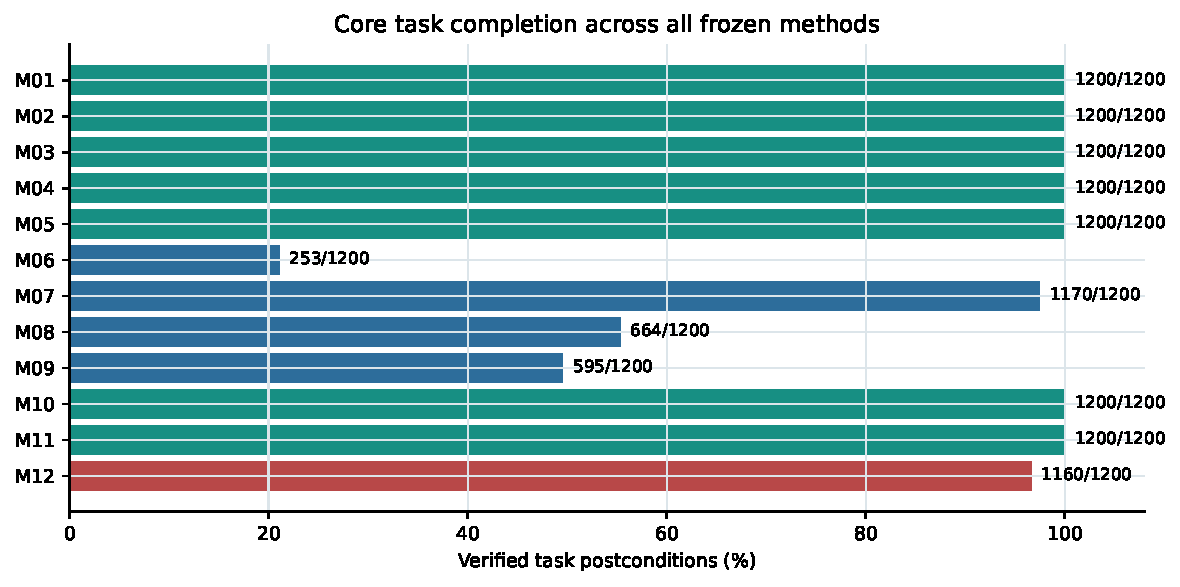
\includegraphics[width=.86\linewidth]{core-success.pdf}\caption{Core completion rates expose a ceiling baseline and the proposed controller lower success count on this authored task suite.}\label{fig:m12-core-success}\end{figure}
\begin{figure}[H]\centering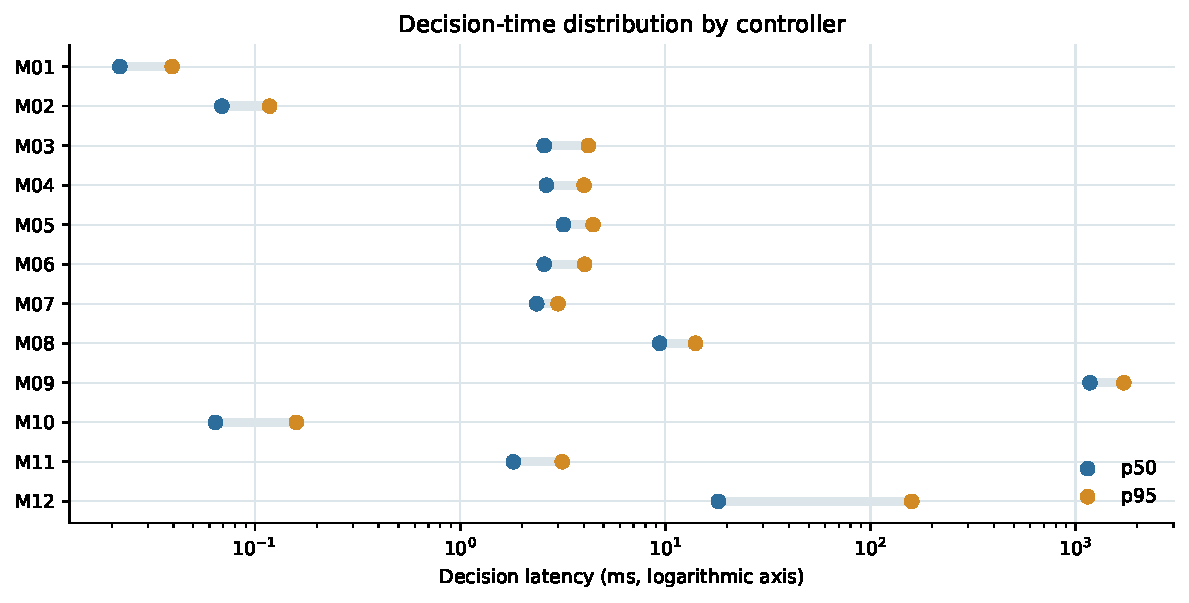
\includegraphics[width=.86\linewidth]{core-latency.pdf}\caption{Median and tail decision latency show the proposed controller's compute cost relative to the guarded finite-state baseline.}\label{fig:m12-latency}\end{figure}
\begin{figure}[H]\centering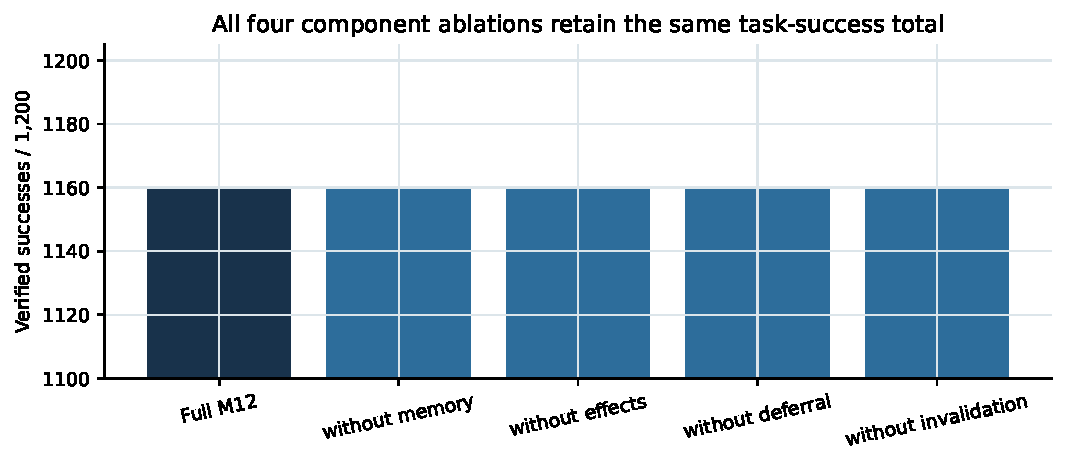
\includegraphics[width=.82\linewidth]{m12-ablations.pdf}\caption{Removing memory, effect information, deferral, or invalidation leaves the measured success count unchanged on the 1,200-episode core set.}\label{fig:m12-ablations}\end{figure}
\begin{figure}[H]\centering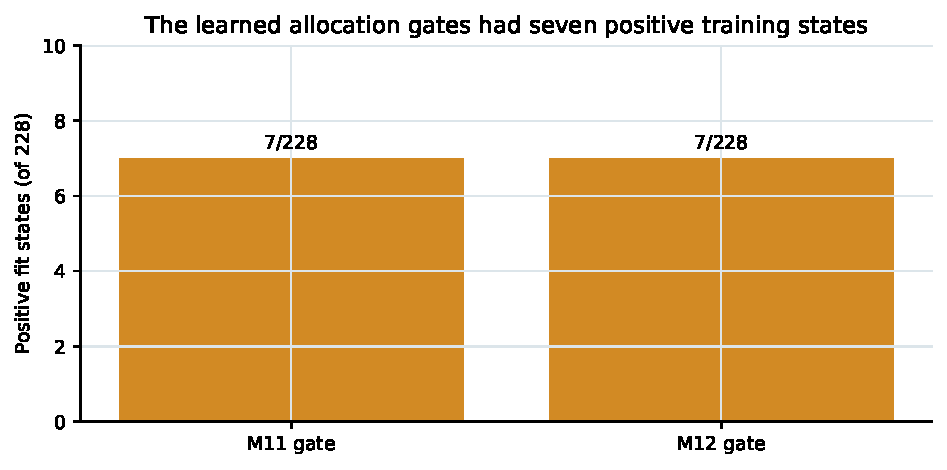
\includegraphics[width=.70\linewidth]{gate-positive-states.pdf}\caption{Only seven positive fit examples inform each allocation gate, which selects a threshold that never delegates.}\label{fig:m12-gate-data}\end{figure}
\begin{figure}[H]\centering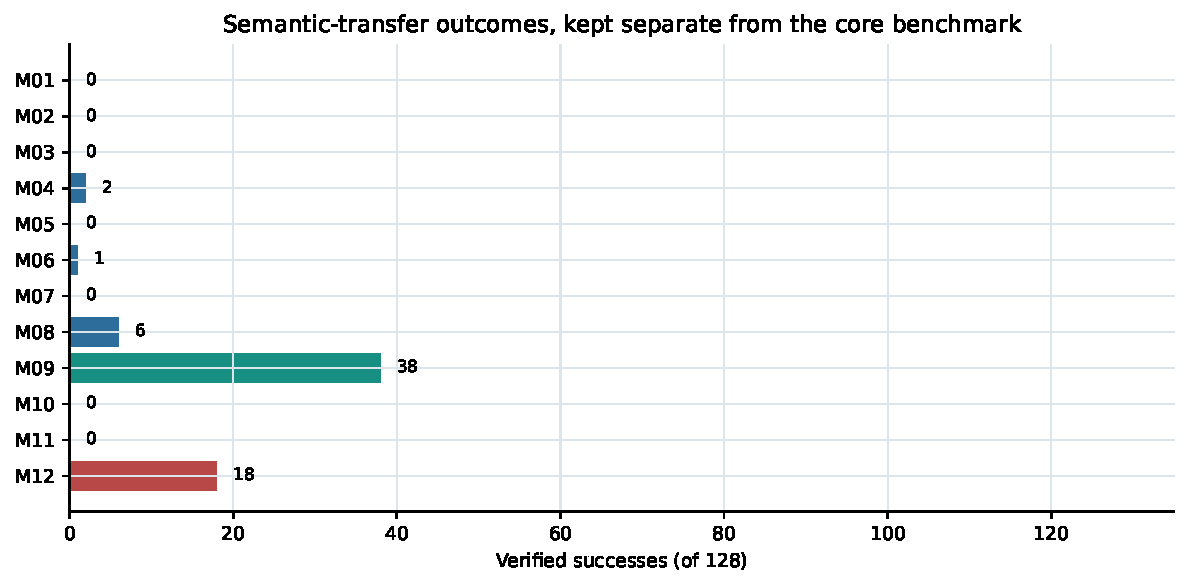
\includegraphics[width=.86\linewidth]{semantic-transfer-success.pdf}\caption{The separate semantic-transfer lane shows M09 above M12 across its 128 matched episodes per method for all reported methods.}\label{fig:m12-transfer}\end{figure}
\begin{figure}[H]\centering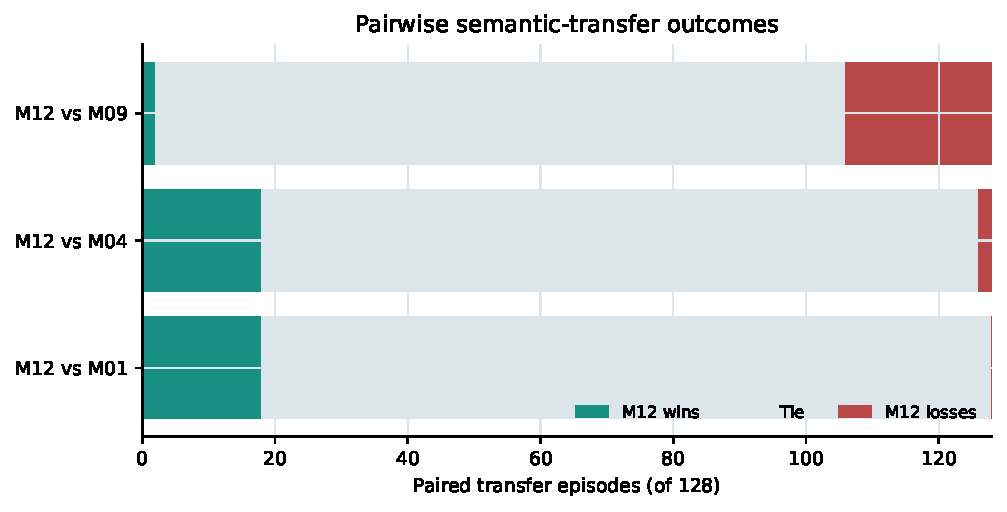
\includegraphics[width=.78\linewidth]{semantic-transfer-pairs.pdf}\caption{Paired outcomes show M12 wins, ties, and losses against selected methods over 128 matched semantic-transfer episodes per method.}\label{fig:m12-transfer-pairs}\end{figure}

Figure~\ref{fig:m12-core-success} shows that the guarded controller reaches the ceiling on this core suite while M12 does not. Figure~\ref{fig:m12-latency} shows the corresponding latency difference on a logarithmic axis; it should not be converted into a universal speed ratio because hardware, warm-up, and workload composition affect the measurements. Figure~\ref{fig:m12-ablations} confirms that the measured task-success aggregate is unchanged by each tested component removal. Figure~\ref{fig:m12-gate-data} explains one limitation of the allocation fit: only seven positive utility labels were available and the selected threshold produces no delegation. Figures~\ref{fig:m12-transfer} and~\ref{fig:m12-transfer-pairs} show that the distinct semantic-transfer lane favors M09 over M12 in this slice.

The 95\% seed-cluster bootstrap interval for M12 core success collapses to 96.67\% because resampling repeats the same within-cell outcomes. It must not be read as evidence that future-family uncertainty is negligible. In the 128 matched semantic-transfer comparisons against M09, M12 wins two, loses 22, and ties 104. The paired loss excess is descriptive of these cases; the eight shared operation families mean these are not 128 independent family replications.

\begin{table}[ht]
\centering\small
\caption{Evaluation populations, measured outcomes, and inference boundaries for the separately reported evidence lanes and denominators.}
\label{tab:evaluation-populations}
\begin{tabularx}{\linewidth}{l r X X}\toprule
Population & Episodes & Construction and observation & Inference boundary \\\midrule
Core & 14,400 & 20 families, six variants, ten seeds and twelve methods & Authored workload; saturated baseline and sparse seed variation \\
Structural transfer & 24 & Held-out compositions; M04 24/24 and M12 21/24 & Small descriptive sample \\
Semantic transfer & 1,536 & Eight opaque-operation families, 128 per method & Separate lane; paired results clustered by family \\
Event-response audit & 4,320 & Post-hoc response, invariant, re-verification and goal checks & Exploratory diagnostic, not confirmatory \\\bottomrule
\end{tabularx}
\end{table}

Table~\\ref{tab:evaluation-populations} preserves each evidence lane and its permitted interpretation. The result index records the status of each frozen episode. A valid hash proves identity with archived bytes, while the independent task checker supplies the outcome. Replay verifies that the same record is read; it is not a fresh experiment. A future run requires a new run identifier, source and package lineage, execution environment, randomization record, and frozen denominator before its outcomes can be compared with these data.

The native runtime audit and task-performance benchmark answer different questions. A separate numerical export check compares selected Rust outputs with Python reference outputs and reports maximum absolute probability error below the declared tolerance for its tested vectors. This supports parity for the tested checkpoint and inputs, not calibration, policy quality, or invariance over all inputs. Likewise, zero declared contract violations among recorded episodes is bounded evidence about those traces, not proof that no malformed or stale proposal can be admitted under every concurrent schedule. Release claims should name the tested methods, checkpoints, vectors, and denominators.

The native runtime audit and task-performance benchmark answer different questions. A separate numerical export check compares selected Rust outputs with Python reference outputs and reports maximum absolute probability error below the declared tolerance for its tested vectors. This supports parity for the tested checkpoint and inputs, not calibration, policy quality, or invariance over all inputs. Likewise, zero declared contract violations among recorded episodes is bounded evidence about those traces, not proof that no malformed or stale proposal can be admitted under every concurrent schedule. Release claims should name tested methods, checkpoints, vectors, and denominators.

\section{Ablation analysis}
The four ablations remove memory, effect information, deferral, or invalidation, with each evaluated on the 1,200-episode core matrix. Every ablation records 1,160 successes, exactly matching full M12, and the paired task-success difference is zero across the 1,200 matched cells. Figure~\ref{fig:m12-ablations} presents these equal aggregates. This result means the current benchmark does not identify a task-success contribution from any removed component. It does not prove the components have no value under conditions that exercise their intended mechanism.

The interpretation is constrained by exposure. If a benchmark has no stale proposal, removing invalidation cannot reveal whether invalidation prevents stale effects. If most tasks can be solved by one deterministic rule, recurrent memory and learned action preference may not alter the terminal checker. If the fitted allocation gate never delegates, removing delegation cannot change the observed policy path. A component can therefore be operationally present but empirically inert on a suite that does not activate its decision boundary. Component claims need mechanism-specific exposure counts as well as end-task success.

For a stronger component study, each ablation must preserve the same initial task, resource state, candidate surface, compute budget, and goal checker. The manipulation should remove one mechanism while holding all else fixed, and the protocol should preregister an outcome on which that mechanism is expected to act: stale-proposal admission for invalidation, effect-prediction residual for effect memory, recurrence-dependent choice after informative history, and incremental utility under calibrated planner outcomes for deferral. Report mechanism exposure, policy decisions, effect records, and terminal outcomes together. The present ablation is limited to task-success equality and does not supply these positive mechanism checks. In particular, a zero difference does not show that the ablated and complete policies are equivalent within a practical margin. Nor does it show that all four mechanisms were invoked equally often: a never-defer allocation gate makes the deferral component inactive by construction. The correct conclusion is that the suite and reported endpoint failed to identify an incremental task-success contribution.

Table~\ref{tab:component-interpretation} separates each component's intended mechanism, observed outcome, and supported inference. A null difference on task success is not proof of equivalence, especially when the relevant trigger is rare or absent. A formal equivalence claim would require a prespecified margin and an experiment powered to distinguish values inside and outside it.
\begin{table}[ht]
\centering\small
\caption{Interpretation of four component removals against mechanism exposure and measured task-success outcomes on the 1,200-episode core suite.}
\label{tab:component-interpretation}
\begin{tabular}{p{.20\linewidth}p{.24\linewidth}p{.22\linewidth}p{.22\linewidth}}\toprule
Removed component & Intended role & Observed evidence & Supported interpretation \\\midrule
Memory & Preserve episode-local history & Same 1,160/1,200 success & No identified contribution on this suite \\
Effect information & Condition updates on observed effects & Same 1,160/1,200 success & No identified contribution on this suite \\
Deferral & Request slower computation when useful & Gate chose never-defer & Benefit not exercised by this fit \\
Invalidation & Reject proposals with stale bindings & Same 1,160/1,200 success & No stale-effect benefit identified by task success \\\bottomrule
\end{tabular}
\end{table}

\section{Discussion}
Table~\ref{tab:invariants} links critical runtime invariants to their enforcement boundary and minimum audit evidence. A conformance suite must contain both passing and failing examples; a test that never mutates a resource cannot establish stale-proposal rejection.
\begin{table}[ht]
\centering\small
\caption{Runtime invariants, enforcing boundaries, and attempted-event evidence for revision-bound action execution in evaluated software tasks.}
\label{tab:invariants}
\begin{tabular}{p{.29\linewidth}p{.23\linewidth}p{.34\linewidth}}\toprule
Invariant & Enforcing boundary & Required evidence \\\midrule
Only current admitted actions execute & Native broker & Attempted denied and stale actions with effect records \\
Planner assumptions remain current & Binding validator and broker & Proposal replay after each bound-field mutation \\
Goal success comes from independent check & Task evaluator & Terminal state and checker result linked by episode identity \\
Unresolved effects are not retried blindly & Reconciliation contract & Timeout, uncertain effect record, and recovery traces \\\bottomrule
\end{tabular}
\end{table}
Table~\ref{tab:invariants} states design obligations; it does not imply a population-level guarantee from the benchmark. Contract and fault-injection evidence must carry attempted-event denominators.
The evidence does not support the prediction that M12 improves task completion or decision efficiency on the tested workload. The guarded finite-state policy solves all core episodes at substantially lower measured decision latency. M12 fails 40 cancellation episodes; its four ablations preserve the same success total; its learned gate selects never-defer; the small structural-transfer slice favors the gradient-boosted policy; and the separate semantic-transfer slice favors M09. These results are negative for the proposed performance claim, even though the method and runtime are implemented.

The version-binding design answers a narrower engineering question: under complete and reliable revisions, canonical serialization, collision resistance, and mandatory final broker admission, a proposal with a mismatched binding should not be executable. This conditional property is not a task-success result and is not established merely by the absence of observed violations in a finite run. Its evidence requires attempted stale proposals and explicit counts by mutation type. Likewise, the native broker's correctness and journal recovery are separate from policy quality. The manuscript keeps these claims distinct because combining them would let infrastructure evidence imply a learning benefit that the data do not show.

The next engineering decision is to change the evaluation conditions, not tune against the saturated test outcomes. A useful study would include controlled ambiguity and environment drift, with prespecified examples where further reasoning changes the independently checked terminal result and counterexamples where delay or incorrect plans hurt. It would sample new task families, vary tool reliability and event timing across seeds, match compute budgets, and hold back families through model fitting and threshold selection. The fast baseline must remain competent and authority-equivalent; making it fail by removing safety checks would not test the allocation hypothesis.

The supported user-facing claim is limited: Neuraxis exposes candidate proposals, admission, effects, revisions and postconditions for inspection and comparison. These data do not establish artificial general intelligence, biological dual-process equivalence, or an M12 advantage. The operational workbench separately uses a deterministic prerequisite policy and should not be represented as live M12 control. A publication should preserve this boundary in its title, abstract, site copy, and figure captions.

This is an implementation-level negative finding with a clear scope. It is not a claim that learned metacontrol cannot work. It states that the available evidence, under the recorded workload and protocol, does not show that this controller improves the measured success and cost outcomes. The negative result can guide a new experiment, but it cannot be repaired by rewording the abstract, adding an architecture illustration, or changing the denominator. A follow-up must add independently varied conditions that create real opportunities for computation to affect verified outcomes, then preserve the same authority and postcondition checks.


\section{Limitations and discriminating experiments}
The core tasks are saturated by M01, making success improvements unidentifiable on most cases. Ten seeds yield identical outcomes in many method-case-variant cells, so episode count overstates independent variation. Only seven positive labels informed the gate. The transfer sample is small. The current evidence therefore cannot support a broad generalization claim.

A discriminating evaluation should create held-out task families with ambiguous specifications, changing tool behavior, conflicting resource revisions, variable planner quality, and costly but recoverable failures. It should include both cases where planning changes the verified outcome and cases where delegation is wasteful or harmful. Train, calibrate, select thresholds, and evaluate on disjoint families. Randomize meaningful transition and tool outcomes across seeds. Match compute budgets; report success, latency, total cost, effect correctness, recovery, invalidation, and planner utilization. Pre-register a minimum effect and uncertainty procedure at the family level. Stress-test stale proposals and cancellation under injected delays. A positive result requires a paired advantage over M01 and M04 without degraded authority or postcondition guarantees. The analysis should report both intention-to-treat outcomes over all scheduled episodes and exposure-conditional diagnostics with their own denominators. Failures caused by missing evidence, invalid actions, tool timeouts, or postcondition failure must remain distinguishable. If a stopping rule is used, it must be fixed before inspecting the held-out outcomes. These decisions prevent a new experiment from recreating the same ambiguity about what the episode count represents.

The test population omits human clarification, long-running repository maintenance, multi-tenant production contention, external service outages, and tasks whose success is judged through evolving user preferences. Each can change the cost of waiting, the value of a tool call, and the meaning of the final goal. They should enter through explicit specifications and versioned contracts before new claims are written. Handling a finite candidate set does not establish understanding of arbitrary files, tools, or intent.

Threats to construct validity include authored workflows standing in for real software tasks and an oracle that may encode a narrow success definition. Internal validity is bounded by method lineage, endpoint stochasticity, and potentially different information timing. Statistical validity is bounded by the small number of independently varying families and sparse positive labels. External validity is limited by absent production repositories, live service dynamics, and human feedback. Hashes protect artifact identity but do not resolve these threats. A follow-up should publish task creation criteria, independent review of the oracle, and a family-level sampling plan before evaluation.

\section{Conclusion}
M12 specifies a software metacontroller that couples fast recurrent action selection with bounded lookahead, outcome-sensitive allocation, asynchronous delegation, and explicit resource-version validation. Its implementation has not demonstrated an advantage on the current benchmark: a guarded finite-state controller is faster and solves every core task, while the proposed controller fails a cancellation subset and its ablations do not change task success. The contribution is a falsifiable method design and a set of benchmark-derived constraints for a more discriminating evaluation. No conclusion about general intelligence or biological equivalence follows.

The evidence-based decision is to withhold superiority claims and design a family-held-out evaluation with meaningful stochastic variation and confirmed opportunities for deliberation to change verified outcomes. Until that test is run, M12 is an implemented approach whose measured benefit remains unestablished. A later positive result would need to replicate across independently sampled families and preserve the action-authority checks that make effect execution auditable.
The method specification remains useful as an executable target for that test: its proposals and assumptions are explicit enough to vary, invalidate, and inspect. It is not an empirically validated allocation principle.

\section*{Data and code availability}
Source code, frozen traces, derived indexes, evaluation scripts, and runtime contracts are available at \url{https://github.com/fsantibanezleal/CAOS_Neuraxis}. The separately versioned engine is available at \url{https://github.com/fsantibanezleal/reflexmesh}. The product-wide methods, protocol, and benchmark analysis are available in the Neuraxis technical report. The committed figures and tables are regenerated from result artifacts with \path{scripts/build_manuscript_figures.py} and \path{scripts/build_manuscript_tables.py}. Before analyzing frozen data, run these validators:
\begin{itemize}
\item \path{scripts/check_artifacts.py} verifies core episode identity, hashes, matrix coverage, and denominators.
\item \path{scripts/check_semantic_transfer.py} verifies the separate transfer lane and matched outcomes.
\item \path{scripts/check_event_responses.py} recomputes the exploratory response analysis from its frozen source episodes.
\end{itemize}
The validators do not modify the frozen episodes. Keep each new evaluation under a distinct run identifier and retain its task specification, task-family split, package versions, planner endpoint, device, and timing measurements. Separate training duration, per-decision latency, and total episode time. The negative result is scoped to the stated tasks, implementation, and evaluation conditions; it does not estimate performance on untested software environments.

\footnotesize
\begin{thebibliography}{99}
\bibitem{daw2005} N. D. Daw, Y. Niv, and P. Dayan. Uncertainty-based competition between prefrontal and dorsolateral striatal systems for behavioral control. \emph{Nature Neuroscience}, 8:1704--1711, 2005. doi:10.1038/nn1560.
\bibitem{lee2014} S. W. Lee, S. Shimojo, and J. P. O'Doherty. Neural computations underlying arbitration between model-based and model-free learning. \emph{Neuron}, 81:687--699, 2014. doi:10.1016/j.neuron.2013.11.028.
\bibitem{kool2016} W. Kool, F. A. Cushman, and S. J. Gershman. When does model-based control pay off? \emph{PLoS Computational Biology}, 12:e1005090, 2016. doi:10.1371/journal.pcbi.1005090.
\bibitem{rao1999} R. P. N. Rao and D. H. Ballard. Predictive coding in the visual cortex. \emph{Nature Neuroscience}, 2:79--87, 1999. doi:10.1038/4580.
\bibitem{mante2013} V. Mante et al. Context-dependent computation by recurrent dynamics in prefrontal cortex. \emph{Nature}, 503:78--84, 2013. doi:10.1038/nature12742.
\bibitem{madras2018} D. Madras, T. Pitassi, and R. Zemel. Predict responsibly: Improving fairness and accuracy by learning to defer. In \emph{NeurIPS}, 2018.
\bibitem{mozannar2020} H. Mozannar and D. Sontag. Consistent estimators for learning to defer to an expert. In \emph{ICML}, 2020. URL: \url{https://proceedings.mlr.press/v119/mozannar20b.html}.
\bibitem{russell1991} S. Russell and E. Wefald. Principles of metareasoning. \emph{Artificial Intelligence}, 49:361--395, 1991.
\bibitem{sutton1999} R. S. Sutton, D. Precup, and S. Singh. Between MDPs and semi-MDPs: A framework for temporal abstraction in reinforcement learning. \emph{Artificial Intelligence}, 112:181--211, 1999. doi:10.1016/S0004-3702(99)00052-1.
\bibitem{dptagent} S. Zhang et al. Leveraging dual process theory in language agent framework for real-time simultaneous human-AI collaboration. In \emph{ACL}, 2025. URL: \url{https://aclanthology.org/2025.acl-long.206/}.
\bibitem{toolsandbox} Y. Lu et al. ToolSandbox: A Stateful, Conversational, Interactive Evaluation Benchmark for LLM Tool Use Capabilities. arXiv:2408.04682, 2024.
\bibitem{react} S. Yao et al. ReAct: Synergizing Reasoning and Acting in Language Models. In \emph{International Conference on Learning Representations}, 2023. URL: \url{https://openreview.net/forum?id=WE_vluYUL-X}.
\bibitem{toolformer} T. Schick et al. Toolformer: Language Models Can Teach Themselves to Use Tools. In \emph{Advances in Neural Information Processing Systems}, 36, 2023. doi:10.52202/075280-2997.
\bibitem{swebench} J. Jimenez et al. SWE-bench: Can Language Models Resolve Real-World GitHub Issues? In \emph{International Conference on Learning Representations}, 2024. URL: \url{https://openreview.net/forum?id=VTF8yNQM66}.
\bibitem{taubench} S. Yao et al. $\tau$-bench: A Benchmark for Tool-Agent-User Interaction in Real-World Domains. arXiv:2406.12045, 2024.
\bibitem{friedman2001} J. H. Friedman. Greedy function approximation: A gradient boosting machine. \emph{The Annals of Statistics}, 29(5):1189--1232, 2001. doi:10.1214/aos/1013203451.
\bibitem{chen2016} T. Chen and C. Guestrin. XGBoost: A scalable tree boosting system. In \emph{Proceedings of the 22nd ACM SIGKDD International Conference on Knowledge Discovery and Data Mining}, pages 785--794, 2016. doi:10.1145/2939672.2939785.
\bibitem{cho2014} K. Cho et al. Learning Phrase Representations using RNN Encoder--Decoder for Statistical Machine Translation. In \emph{Proceedings of EMNLP}, pages 1724--1734, 2014. doi:10.3115/v1/D14-1179.
\bibitem{li2010} L. Li, W. Chu, J. Langford, and R. E. Schapire. A contextual-bandit approach to personalized news article recommendation. In \emph{Proceedings of the 19th International Conference on World Wide Web}, pages 661--670, 2010. doi:10.1145/1772690.1772758.
\bibitem{schulman2017} J. Schulman et al. Proximal Policy Optimization Algorithms. arXiv:1707.06347, 2017.
\bibitem{suttonbarto2018} R. S. Sutton and A. G. Barto. \emph{Reinforcement Learning: An Introduction}. 2nd edition, MIT Press, 2018. URL: \url{http://incompleteideas.net/book/the-book-2nd.html}.
\bibitem{efron1993} B. Efron and R. J. Tibshirani. \emph{An Introduction to the Bootstrap}. Chapman \& Hall, 1993. URL: \url{https://doi.org/10.1201/9780429246593}.
\bibitem{demsar2006} J. Dem\v{s}ar. Statistical comparisons of classifiers over multiple data sets. \emph{Journal of Machine Learning Research}, 7:1--30, 2006. URL: \url{https://jmlr.org/papers/v7/demsar06a.html}.
\bibitem{nadeau2003} C. Nadeau and Y. Bengio. Inference for the generalization error. \emph{Machine Learning}, 52:239--281, 2003. doi:10.1023/A:1024068626366.
\bibitem{guo2017} C. Guo, G. Pleiss, Y. Sun, and K. Q. Weinberger. On calibration of modern neural networks. In \emph{Proceedings of the 34th International Conference on Machine Learning}, PMLR 70:1321--1330, 2017. URL: \url{https://proceedings.mlr.press/v70/guo17a.html}.
\end{thebibliography}
\end{document}
